\subsection{Regulación de sistemas lineales: caso 1}

Cuando no hay integrador en la planta, es decir todos los polos son distintos de cero, el sistema en lazo cerrado no alcanza la referencia, por ello Se añade una ganancia en la referencia.
Considerando el sistema en lazo cerrado
\[(1)
    \left\{
        \begin{array}{lll}
            \dot{x}(t) = (A-Bk)x(t) + B\underbrace{r(t)}_{u(t)} \\
            y(t) = Cx(t)
        \end{array}
    \right.
\]

considerando que el sistema (1) tiene inicialmente una ganancia de 1, es decir, la función de transferencia es
\[
    \frac{y(s)}{u(s)} = C(sI-(A-Bk))^{-1}B = 1
\]

Se le agrega una ganancia \( N \) tal que
\[
    \frac{y(s)}{u(s)N} = C(sI-(A-Bk))^{-1}B = \frac{1}{N}
\]

o bien
\[
    \frac{y(s)}{u(s)} = NC(sI-(A-Bk))^{-1}B = 1 \\
\]

\begin{figure}[h!]
    \centering
        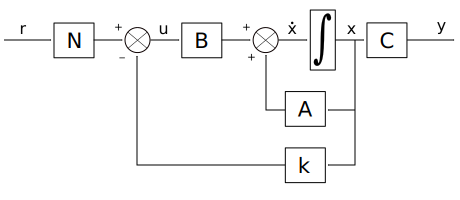
\includegraphics[scale=0.20]{Control de Sistemas Mecatronicos Figuras/14 Ganancia de precompensacion.png}
        \caption{Ganancia de precompensación}
\end{figure}

Para una entrada \( r \) constante, en estado estacionario se tiene que 
\[
    \begin{split}
        \lim_{t \to \inf}(\frac{y(s)}{u(s)}) & = NC(A-Bk)^{-1}B = 1 \\
        N & = \frac{1}{C(A-Bk)^{-1}B}
    \end{split}
\]

Usando la representación con polos y ceros
\[
    \begin{split}
        \lim_{t \to \inf}(\frac{y(s)}{u(s)}) & = N \frac{ b_{1}s^{n-1} + \ldots + b_{n} }{ s^{n} + a_{1}s^{n-1} +\ldots + a_{n} } = 1 \\
        N \frac{b_{n}}{a_{n}} & = 1 \\
        N & = \frac{a_{n}}{b_{n}}
    \end{split}
\]

Por lo tanto
\[
    N = \frac{1}{C(A-Bk)^{-1}B} = \frac{a_{n}}{b_{n}}
\]

Se consigue reducir el error de estado estacionario a cero, pero debido a que no tiene un integrador, el sistema no responde correctamente ante ruido.